\documentclass{article} 
\usepackage{xcolor} 

%% Page Margins %%
\usepackage{geometry}
\geometry{
    top = 0.75in,
    bottom = 0.75in,
    right = 0.75in,
    left = 0.75in,
}

\usepackage{amsmath}
\usepackage{graphicx}
\usepackage{parskip}

\title{Lab 4: Synchronous Sequential Circuits}

\author{\textcolor{blue}{Tyseer Toufiq}}

\begin{document}
\maketitle

\section*{Part I}

\begin{enumerate}
\setcounter{enumi}{1}
\item Export the subcircuit schematic as an image and include it in your report.

\begin{figure}[ht!]
    \centering
    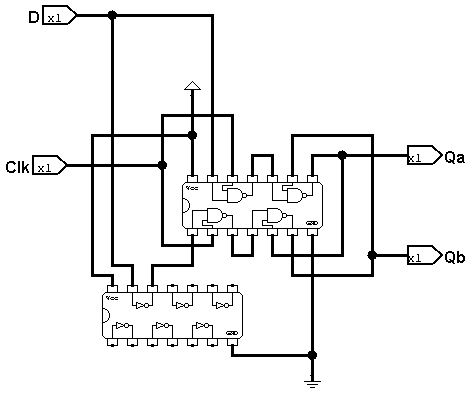
\includegraphics[width=0.5\textwidth]{D-latch.png}
    \caption{A schematic of the gated D-latch.}
    \label{gateddlatch}
\end{figure}


\begin{figure}[ht!]
    \centering
    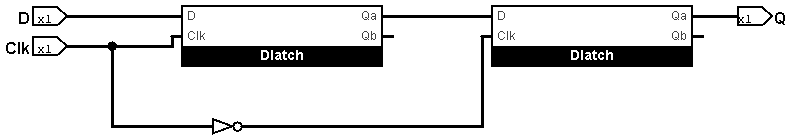
\includegraphics[width=0.5\textwidth]{flip-flop.png}
    \caption{A schematic of the D flip-flop.}
    \label{dflipdlop}
\end{figure}


\item For the D latch and the flip flop, are there any input combinations of Clk and D that should NOT be the first you test with the \emph{Poke} tool? List them if applicable. 
\textcolor{blue}{ 
\\
When we are testing the gated D latch we should first ensure that the clock is set to ON while toggling the input for D. This is because the latch requires the clock to be active/ high at least once to capture and reflect the D input on the output. This then sets the output, which can then hold its state when the clock is subsequently set to low. In other words, these combinations cause undefined outputs because the initial values of Qa and Qb are set yet}
\end{enumerate}

\section*{Part IIa}

\begin{enumerate}
\setcounter{enumi}{1}
\item Export the subcircuit schematic as an image and include it in your report.

\begin{figure}[ht!]
    \centering
    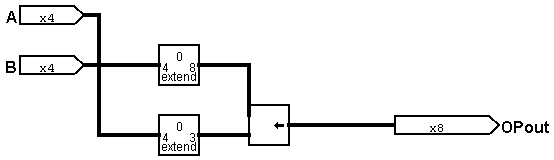
\includegraphics[width=0.4\textwidth]{lab4_op5.png}
    \caption{A schematic of op5.}
    \label{f:op5}
\end{figure}

\begin{figure}[ht!]
    \centering
    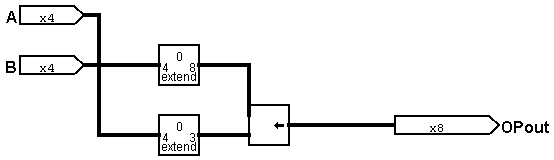
\includegraphics[width=0.4\textwidth]{lab4_op6.png}
    \caption{A schematic of op6.}
    \label{f:op6}
\end{figure}

\begin{figure}[ht!]
    \centering
    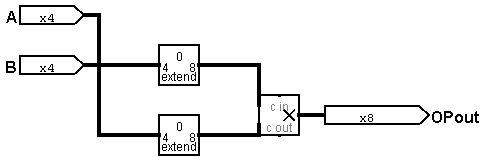
\includegraphics[width=0.4\textwidth]{lab4_op7.png}
    \caption{A schematic of op7.}
    \label{f:op7}
\end{figure}

\item Include a screenshot of your simulated test vectors for op5, op6, and op7.

\begin{figure}[ht!]
    \centering
    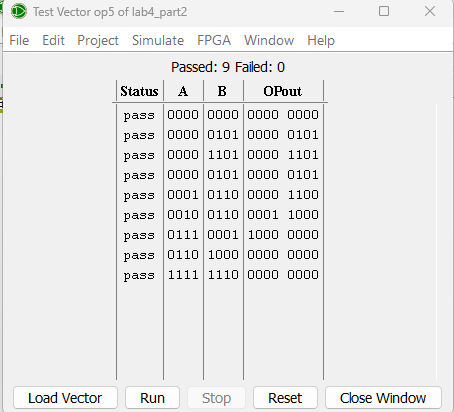
\includegraphics[width=0.4\textwidth]{lab4_op5_simulation.png}
    \caption{A simulation of op5.}
    \label{f:op5_simulation}
\end{figure}

\begin{figure}[ht!]
    \centering
    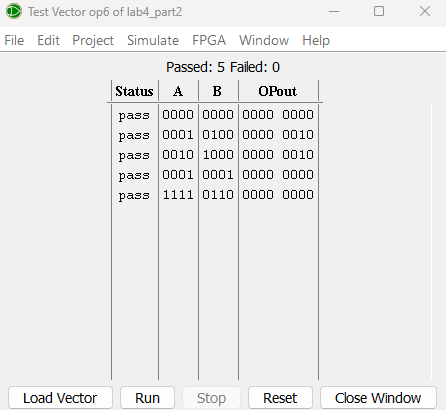
\includegraphics[width=0.4\textwidth]{lab4_op6_simulation.png}
    \caption{A simulation of op6.}
    \label{f:op6_simulation}
\end{figure}

\begin{figure}[ht!]
    \centering
    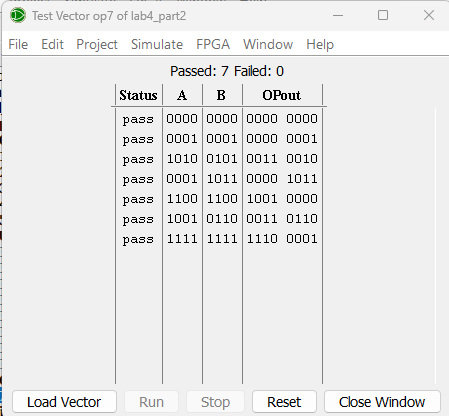
\includegraphics[width=0.4\textwidth]{lab4_op7_simulation.png}
    \caption{A simulation of op7.}
    \label{f:op7_simulation}
\end{figure}


\end{enumerate}

\section*{Part IIb}

\begin{enumerate}
\setcounter{enumi}{2}
\item Include a screenshot of your simulated timing diagram demonstrating ALUreg starting at 0x0 and increasing by 1 until 0x0f.

\begin{figure}[ht!]
    \centering
    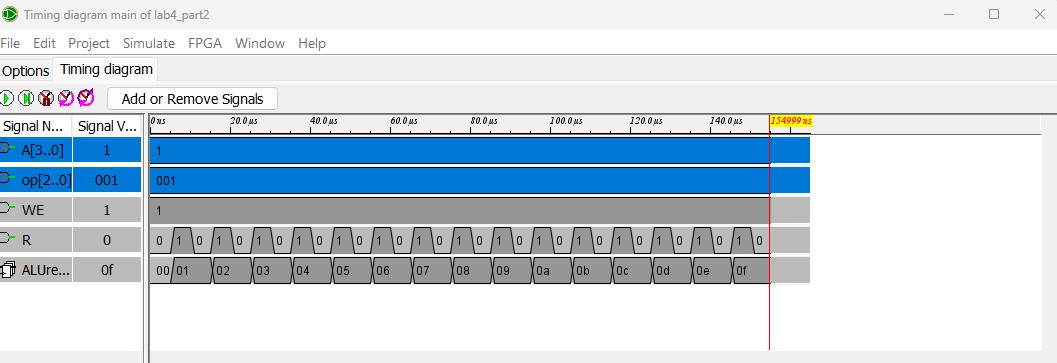
\includegraphics[width=0.4\textwidth]{lab4_timing_plus_one.png}
    \caption{A timing simulation demonstrating incrementing.}
    \label{f:timing_plus_one}
\end{figure}

\item Include a screenshot of your simulated timing diagram demonstrating a shifting operation where ALUreg goes from at 0x01 and doubling until 0x00.

\begin{figure}[ht!]
    \centering
    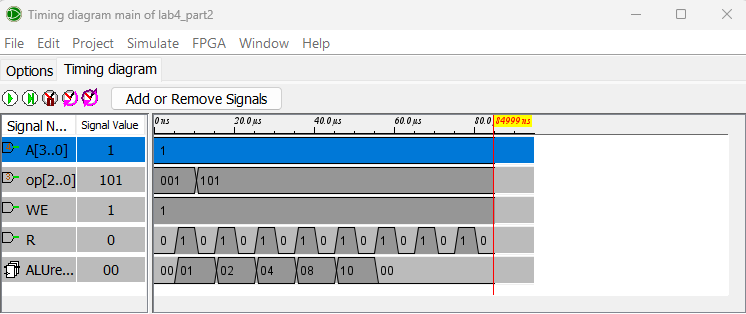
\includegraphics[width=0.4\textwidth]{lab4_timing_times_two.png}
    \caption{A timing simulation demonstrating doubling.}
    \label{f:timing_double}
\end{figure}
\end{enumerate}

\section*{Part III}

\begin{enumerate}
\setcounter{enumi}{1}
\item What is the behavior of the 8-bit shift register when \textit{Load\_n = 1} and \textit{ShiftRight = 0}? Briefly explain in your prelab.  
\textcolor{blue}{ 
When load\_n is 1 and ShiftRight is = 0 the register, nothing will change. This is because load is active and it will not do its task when its 1. ShiftRight is 0 so no shifting will happen so this results in nothing happening in general.}

\item Export the subcircuit schematic as an image and include it in your report.

\begin{figure}[ht!]
    \centering
    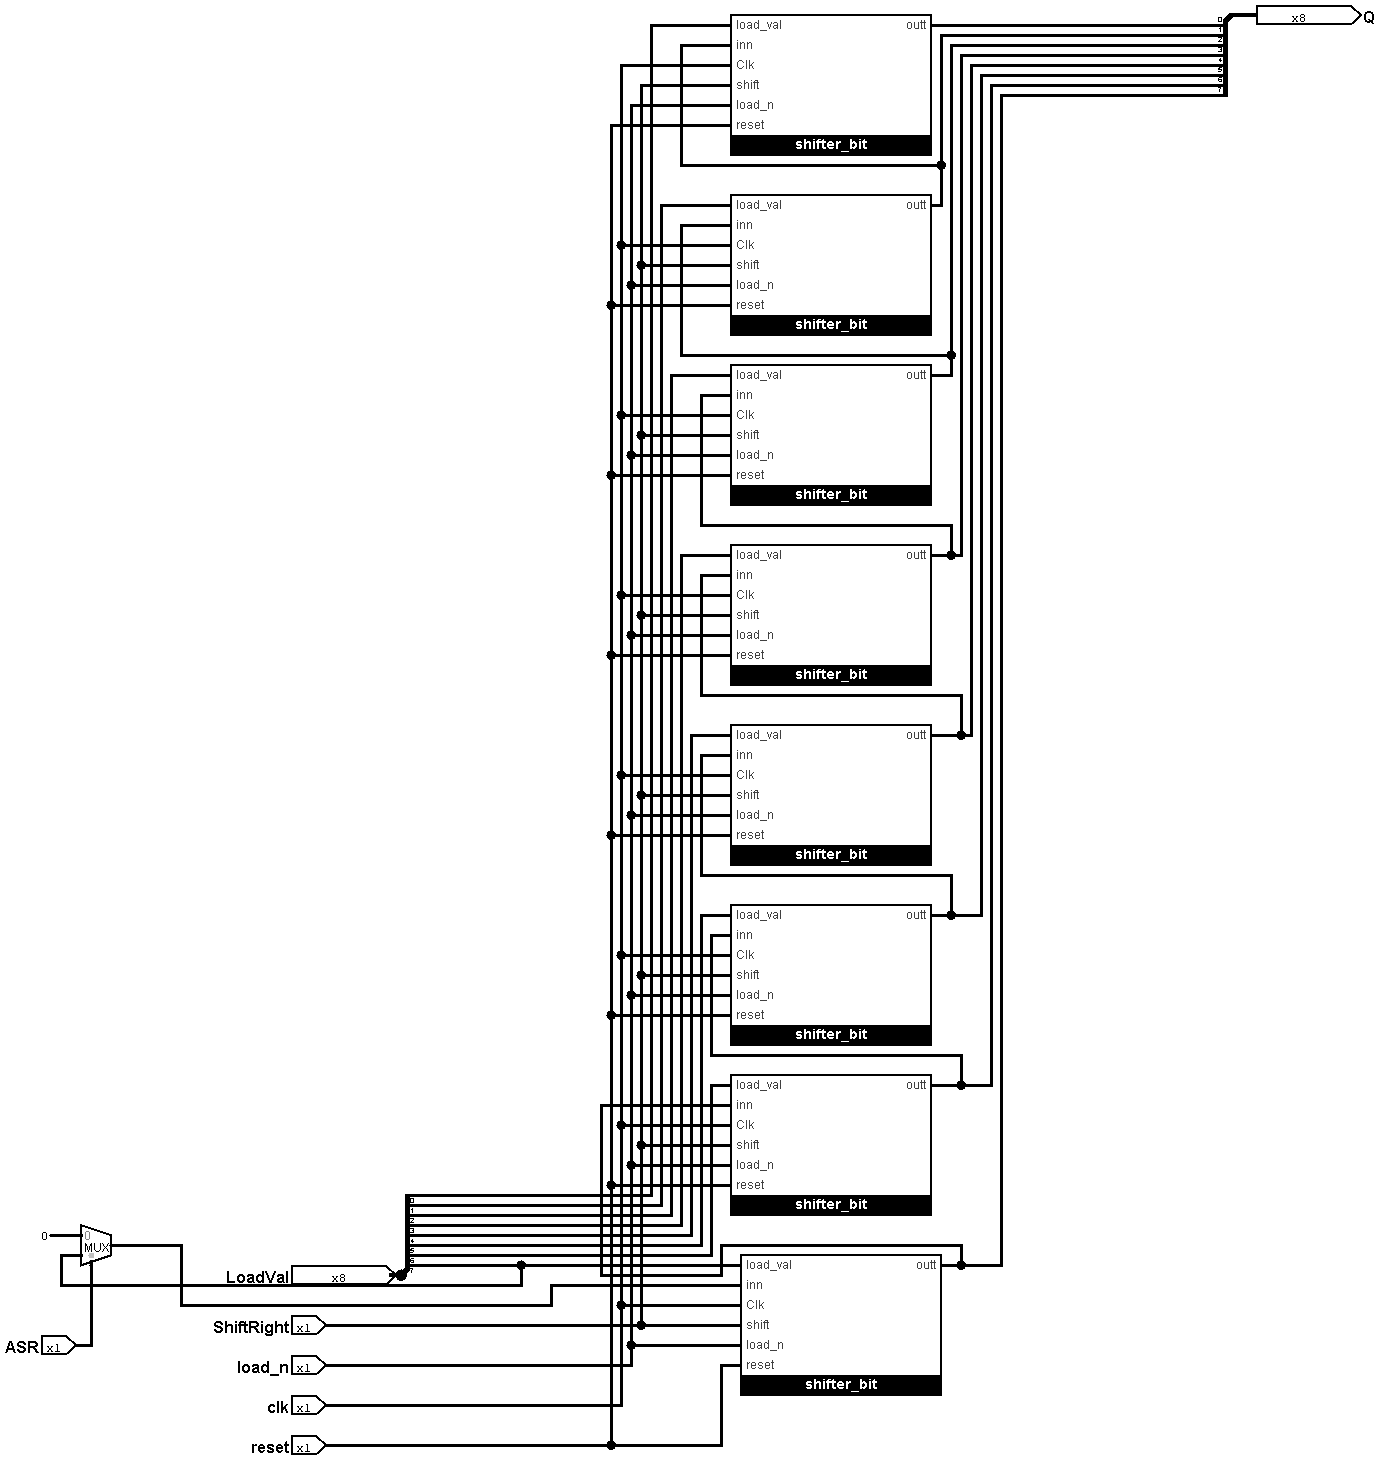
\includegraphics[width=0.5\textwidth]{lab4_shifter_bit.png}
    \caption{A schematic of the 8-bit shift register.}
    \label{f:shifter_bit}
\end{figure}

% \item Include a screenshot of your simulated timing diagram demonstrating that the output can take on values from either input.

\begin{figure}[ht!]
    \centering
    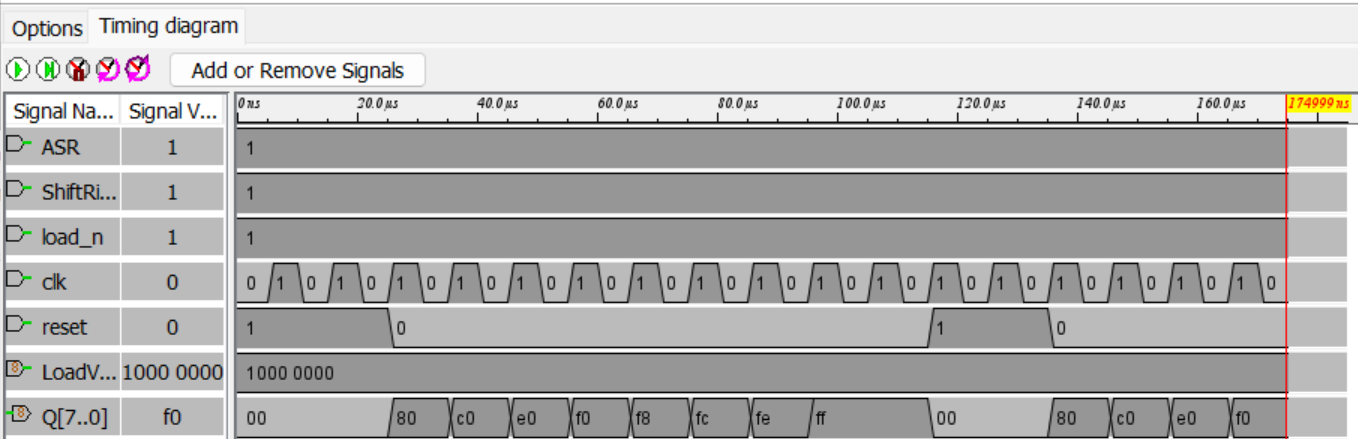
\includegraphics[width=0.5\textwidth]{lab4_shifter_test_1.png}
    \caption{8-bit shift register's test case \#1}
    \label{f:timing_shifter_bit1}
\end{figure}

\begin{figure}[ht!]
    \centering
    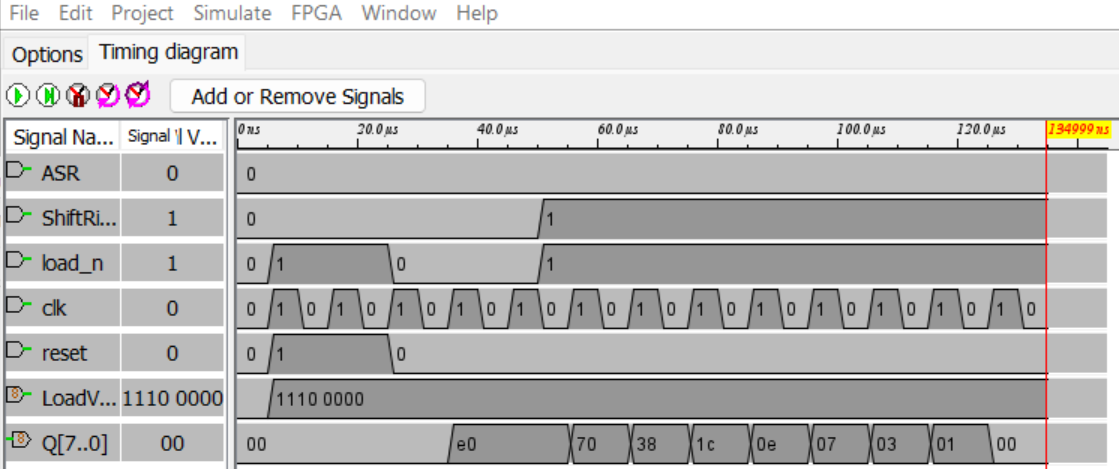
\includegraphics[width=0.5\textwidth]{lab4_shifter_test_2.png}
    \caption{8-bit shift register's test case \#2}
    \label{f:timing_shifter_bit2}
\end{figure}

\begin{figure}[ht!]
    \centering
    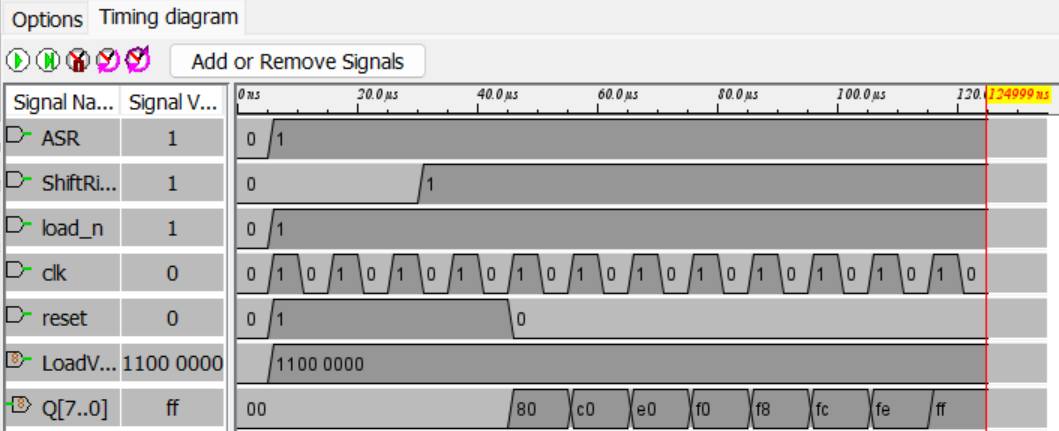
\includegraphics[width=0.5\textwidth]{lab4_shifter_test_3.png}
    \caption{8-bit shift register's test case \#3}
    \label{f:timing_shifter_bit3}
\end{figure}


\end{enumerate}

\end{document}